\documentclass[11pt,a4paper]{article}
\usepackage[margin=1in]{geometry}
\usepackage{amsmath,amssymb,amsfonts}
\usepackage{graphicx}
\usepackage{booktabs}
\usepackage{array}
\usepackage{float}
\usepackage{hyperref}
\usepackage{xcolor}

\graphicspath{{../outputs/figures/}}

\title{Lightweight Hybrid Quantum-Classical Networks for Biomedical Tabular Binary Classification:\\
A Knowledge Distillation and Quantum Layer Placement Study}

\author{Xiaoming Liu\\
Panda Intelligence Software LTD, United Kingdom\\
\texttt{i@pandacat.ai}}

\date{}

\begin{document}
\maketitle

\begin{abstract}
Hybrid quantum-classical architectures provide a practical route for studying quantum components under
NISQ-era resource constraints, but their value on small biomedical tabular problems remains unclear.
We study a lightweight teacher-student pipeline that combines PCA-based feature compression, a compact
classical student, and a 4-qubit parameterized quantum layer. We compare classical and hybrid students
with and without knowledge distillation (KD), and we further ablate quantum layer placement and PCA
dimension on the Breast Cancer Wisconsin Diagnostic dataset using 5-fold cross-validation.
Experimental results show that the hybrid student with KD reaches AUC $0.9931 \pm 0.0054$, matching the
KD classical student in AUC, while the hybrid student without KD achieves the best hybrid F1
($0.9442 \pm 0.0220$). However, the hybrid models require $276$--$330$ seconds per fold (KD to no-KD),
compared with less than one second for the classical students, so the performance gains are not
sufficient to justify the extra simulation cost on this dataset. Ablation experiments show that front
placement of the quantum layer fails severely due to out-of-range angle encoding, whereas middle and
tail placement remain competitive; PCA dimensions 6--8 improve F1/MCC over 4 dimensions, with 6
dimensions offering the best AUC-cost balance. These results suggest that lightweight hybrid models are
feasible for biomedical tabular learning, but careful placement and compression design matter more than
simply adding a quantum layer.
\end{abstract}

\section{Introduction}
\label{sec:intro}

Quantum machine learning (QML) continues to attract interest as a possible route toward practical
learning systems on near-term quantum hardware. In practice, however, large quantum circuits remain hard
to optimize and expensive to simulate, especially in data regimes where strong classical baselines are
already available~\cite{cerezo2021vqa}. Hybrid quantum-classical (HQC) models therefore remain the most
realistic design pattern: a classical front-end performs feature compression, while a small parameterized
quantum circuit (PQC) acts as a learnable nonlinear block~\cite{schuld2021machine}.

Biomedical tabular classification is a useful setting for testing this idea. Such datasets are often
small, feature-limited after preprocessing, and measured under strict performance-cost constraints. A
compact HQC model may therefore provide insight into how and where a quantum block can be inserted,
even if no quantum advantage is expected. At the same time, knowledge distillation (KD) offers a natural
mechanism for transferring supervision from a larger classical teacher to a smaller classical or hybrid
student~\cite{kd}.

This paper asks three concrete questions on the WDBC benchmark:
\begin{enumerate}
\item Does KD help a hybrid quantum-classical student?
\item Where should the quantum layer be placed inside the student network?
\item Is the hybrid student worth its simulation cost relative to a lightweight classical student?
\end{enumerate}

Our contributions are straightforward. First, we benchmark classical and hybrid students under the same
5-fold protocol with a classical teacher baseline. Second, we ablate quantum layer placement and PCA
dimension. Third, we report both predictive quality and training cost, making the trade-off visible
rather than relying on accuracy alone.

\section{Related Work}
\label{sec:rw}

\subsection{Hybrid Quantum-Classical Classification}
Hybrid quantum-classical models couple classical feature extractors with shallow PQCs to keep the quantum
component small enough for near-term simulation or
deployment~\cite{cerezo2021vqa,schuld2021machine}. Prior work has explored this idea for image, text,
and tabular settings, but biomedical tabular benchmarks remain comparatively underused despite their
natural low-dimensional structure after feature selection or
PCA~\cite{sagingalieva2023hyperparameter}.

\subsection{Knowledge Distillation for Quantum Models}
KD transfers information from a stronger teacher to a smaller student through softened targets and has
become a standard compression tool in classical deep learning~\cite{kd}. Recent QML work has extended
KD to classical-to-quantum and quantum-to-quantum transfer settings, arguing that a stable classical
teacher can regularize difficult hybrid optimization~\cite{nguyen2022classicalquantum}.

\subsection{Biomedical Tabular Classification}
Biomedical tabular tasks typically involve limited sample size, moderate class imbalance, and a need for
interpretable, compact models. PCA-based compression is especially relevant when quantum inputs must be
bounded by the number of available qubits~\cite{sagingalieva2023hyperparameter}. This makes WDBC a
suitable benchmark for controlled HQC experiments.

\section{Method}
\label{sec:method}

\subsection{Problem Setup}
Given a binary biomedical tabular dataset $\mathcal{D}=\{(\mathbf{x}_i, y_i)\}_{i=1}^{N}$ with
$y_i \in \{0,1\}$ and $\mathbf{x}_i \in \mathbb{R}^d$, we aim to learn a compact classifier that keeps
predictive quality high while reducing model size and simulation cost.

\subsection{Preprocessing}
Within each training fold, we apply standard scaling followed by PCA to a target dimension
$d' \in \{4,6,8\}$. All preprocessing is fit on the training split only and then applied to the
validation split to avoid data leakage. The default experiments use $d'=4$.

\subsection{Teacher and Student Models}
The teacher is a classical multilayer perceptron with hidden dimensions $[64,32]$ and dropout $0.2$.
The classical student uses hidden dimensions $[16,8]$.

The hybrid student contains three stages:
\begin{enumerate}
\item a classical projection network,
\item a quantum layer with 4 qubits and 1 variational layer,
\item a classical output head producing a binary logit.
\end{enumerate}
We evaluate three insertion positions for the quantum block: front, middle, and tail.

\subsection{Quantum Layer}
The quantum block uses PennyLane's \texttt{AngleEmbedding} with $Y$ rotations followed by
\texttt{BasicEntanglerLayers}~\cite{pennylane}. For 4 qubits and 1 variational layer, the effective
circuit depth is 2 (embedding + one entangling block). The circuit returns 4 Pauli-$Z$ expectation
values that are passed to the classical head.

\subsection{Knowledge Distillation}
The student objective combines a hard-label BCE term with a soft-target distillation term:
\begin{equation}
\mathcal{L} = (1-\lambda)\,\mathcal{L}_{\text{hard}} + \lambda T^2 \mathcal{L}_{\text{KD}},
\end{equation}
where $T$ is the distillation temperature and $\lambda$ is the KD weight. In the main KD runs we use
$T=2$ and $\lambda=0.5$.

\subsection{Evaluation Protocol}
All reported numbers are mean $\pm$ standard deviation over stratified 5-fold cross-validation. We use
AUC, F1, accuracy, MCC, and per-fold training time as the primary evaluation metrics.

\section{Experiments}
\label{sec:exp}

\subsection{Dataset}
The Breast Cancer Wisconsin (Diagnostic) dataset~\cite{wdbc} contains 569 samples, 30 continuous
features, and binary labels with 212 malignant and 357 benign cases. There are no missing values.

\begin{table}[t]
\caption{Dataset statistics.}
\label{tab:data}
\centering\small
\begin{tabular}{lc}
\toprule
Property & Value \\
\midrule
Samples & 569 \\
Raw features & 30 \\
PCA dimensions evaluated & 4 / 6 / 8 \\
Positive class (malignant) & 212 (37.3\%) \\
Negative class (benign) & 357 (62.7\%) \\
Missing values & 0 \\
Task & Binary classification \\
\bottomrule
\end{tabular}
\end{table}

\subsection{Main Results}

\begin{table}[t]
\caption{Main results on WDBC (5-fold CV, PCA $d'=4$). Teacher results are included as an upper-bound reference.}
\label{tab:main}
\centering\small
\begin{tabular}{lcccc}
\toprule
Model & AUC & F1 & MCC & Train Time (s/fold) \\
\midrule
Teacher (MLP-64-32) & $0.9939 \pm 0.0054$ & $0.9416 \pm 0.0155$ & -- & $0.31 \pm 0.01$ \\
\midrule
Student-Classic & $0.9943 \pm 0.0059$ & $0.9432 \pm 0.0277$ & $0.9126 \pm 0.0418$ & $0.22 \pm 0.04$ \\
Student-Classic-KD & $0.9931 \pm 0.0060$ & $0.9419 \pm 0.0212$ & $0.9094 \pm 0.0350$ & $0.50 \pm 0.00$ \\
Student-Hybrid-NoKD & $0.9896 \pm 0.0105$ & $0.9442 \pm 0.0220$ & $0.9129 \pm 0.0343$ & $330.46 \pm 82.43$ \\
Student-Hybrid-KD & $0.9931 \pm 0.0054$ & $0.9395 \pm 0.0152$ & $0.9057 \pm 0.0249$ & $276.46 \pm 21.33$ \\
\bottomrule
\end{tabular}
\end{table}

Table~\ref{tab:main} shows that the classical student is already very strong on WDBC, closely matching
the teacher in AUC despite being four times smaller. The hybrid student without KD slightly trails the
classical student in AUC but matches it in F1 and MCC. Adding KD to the hybrid student raises AUC from
$0.9896$ to $0.9931$ and reduces mean training time by about 16\%, but slightly reduces F1 and MCC.
KD does not improve the classical student on this benchmark: the classical student is already saturating
the task, leaving little residual signal in the teacher's soft targets.

\begin{figure}[t]
\centering
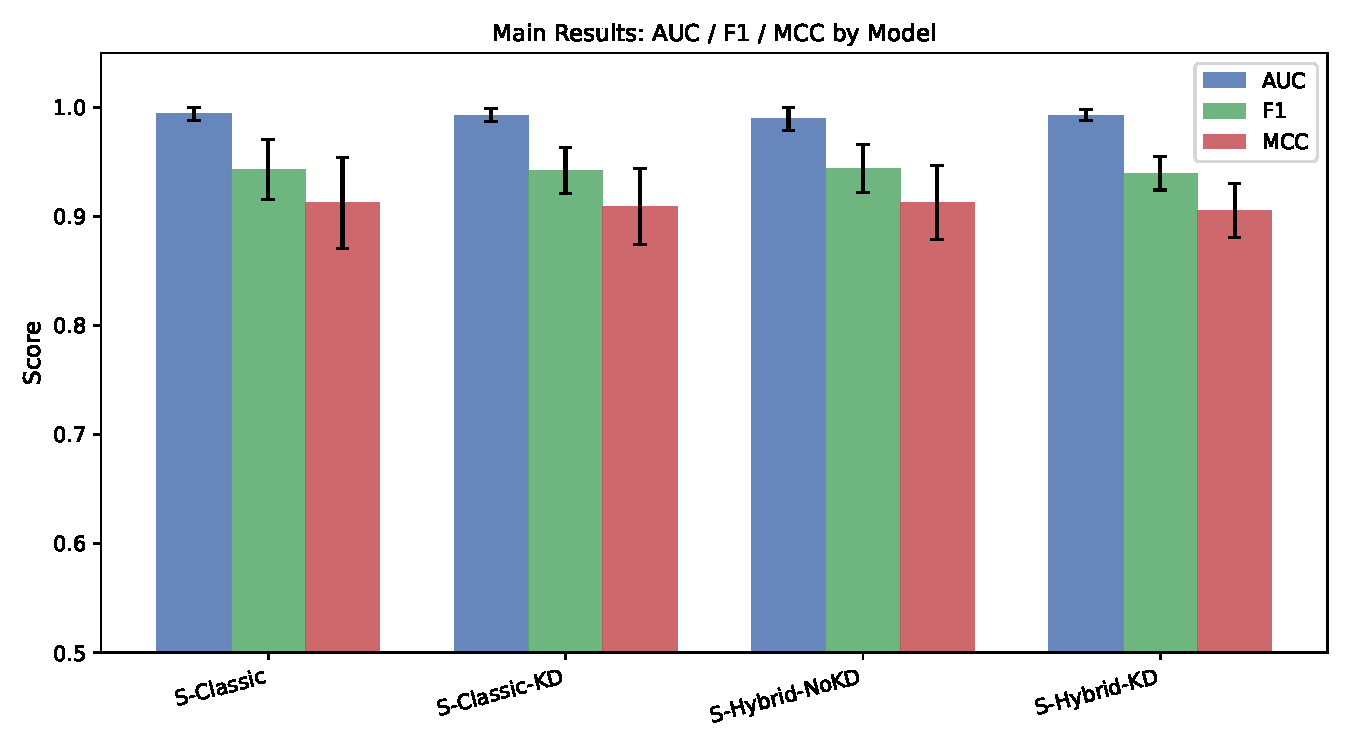
\includegraphics[width=0.92\linewidth]{main_comparison.pdf}
\caption{Main comparison of AUC, F1, and MCC across the four student configurations.}
\label{fig:main_comparison}
\end{figure}

\begin{figure}[t]
\centering
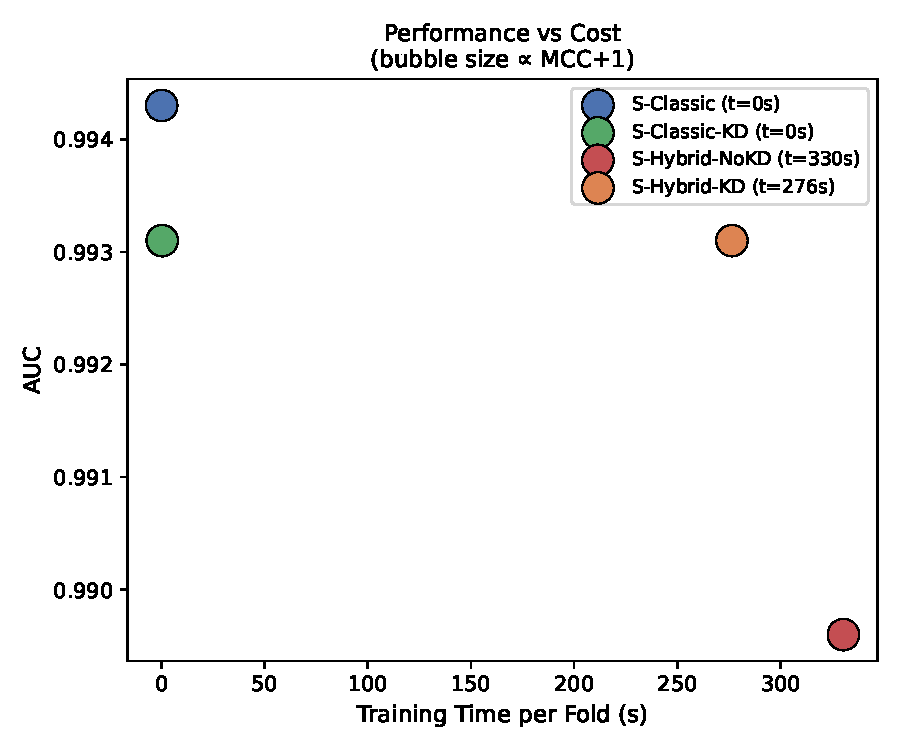
\includegraphics[width=0.82\linewidth]{performance_cost.pdf}
\caption{Performance-cost trade-off. Bubble size is proportional to MCC. Hybrid models occupy a much
higher training-cost region than the classical students.}
\label{fig:perf_cost}
\end{figure}

\subsection{Ablation: Quantum Layer Position}

\begin{table}[t]
\caption{Ablation of quantum layer placement for the KD hybrid student.}
\label{tab:ablation_pos}
\centering\small
\begin{tabular}{lccccc}
\toprule
Position & AUC & F1 & MCC & Train Time (s/fold) & Circuit Depth \\
\midrule
Front  & $0.6721 \pm 0.0638$ & $0.0560 \pm 0.1120$ & $0.0577 \pm 0.1154$ & $226.78 \pm 3.95$ & 2 \\
Middle & $0.9894 \pm 0.0089$ & $0.9510 \pm 0.0262$ & $0.9236 \pm 0.0420$ & $384.56 \pm 35.80$ & 2 \\
Tail   & $0.9903 \pm 0.0073$ & $0.9504 \pm 0.0187$ & $0.9240 \pm 0.0277$ & $347.34 \pm 68.03$ & 2 \\
\bottomrule
\end{tabular}
\end{table}

The placement study in Table~\ref{tab:ablation_pos} reveals the most critical design choice in this
paper. Front placement collapses predictive quality: the raw PCA features are not bounded to
$[-\pi, \pi]$ before angle encoding, so the \texttt{AngleEmbedding} rotations wrap around and lose
discriminative structure, effectively randomizing the quantum state and causing the model to collapse
to a near-constant predictor. Middle and tail placement both avoid this failure because a preceding
classical projection with \texttt{Tanh} activation bounds inputs before encoding.
Tail placement yields the best AUC and MCC, while middle placement gives the best F1. Because tail
placement is also faster on average than middle, it provides the strongest overall placement trade-off.

\begin{figure}[t]
\centering
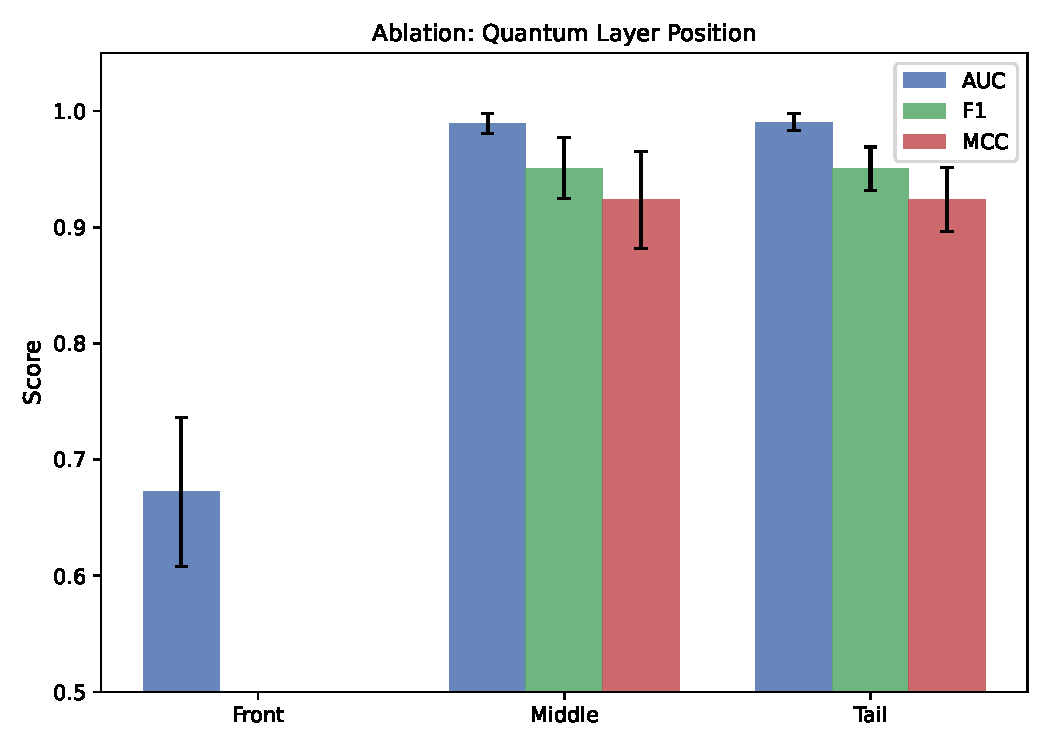
\includegraphics[width=0.88\linewidth]{ablation_position.pdf}
\caption{Effect of quantum layer placement. Front placement collapses due to unbounded angle encoding;
middle and tail remain high-performing.}
\label{fig:ablation_position}
\end{figure}

\subsection{Ablation: PCA Dimension and Distillation Temperature}

\begin{table}[t]
\caption{Ablation of PCA dimension and KD temperature for the KD hybrid student.}
\label{tab:ablation_pca}
\centering\small
\begin{tabular}{llccc}
\toprule
Setting & Value & AUC & F1 & MCC \\
\midrule
PCA dim & 4 & $0.9924 \pm 0.0088$ & $0.9423 \pm 0.0191$ & $0.9103 \pm 0.0300$ \\
PCA dim & 6 & $0.9926 \pm 0.0072$ & $0.9538 \pm 0.0175$ & $0.9283 \pm 0.0274$ \\
PCA dim & 8 & $0.9888 \pm 0.0108$ & $0.9668 \pm 0.0119$ & $0.9488 \pm 0.0178$ \\
$T$ & 2 & $0.9929 \pm 0.0073$ & $0.9442 \pm 0.0228$ & $0.9127 \pm 0.0367$ \\
$T$ & 4 & $0.9932 \pm 0.0060$ & $0.9331 \pm 0.0390$ & $0.9004 \pm 0.0528$ \\
\bottomrule
\end{tabular}
\end{table}

Increasing the PCA dimension from 4 to 6 or 8 improves F1 and MCC substantially. The 8-dimensional
setting achieves the strongest F1 and MCC, but 6 dimensions provides the best balanced operating point
because it preserves the strongest AUC while still improving the other metrics. The temperature ablation
shows that $T=4$ gives a marginally higher AUC, but $T=2$ is preferable overall because it yields
better F1 and MCC with less variance.

\begin{figure}[t]
\centering
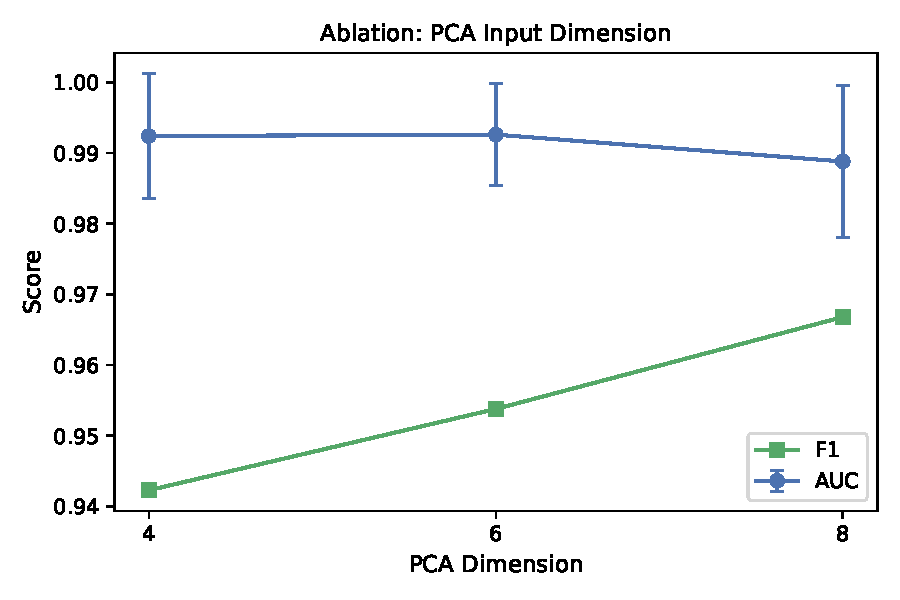
\includegraphics[width=0.82\linewidth]{ablation_pca.pdf}
\caption{Effect of PCA input dimension. Larger compressed inputs improve F1/MCC, with 6 dimensions
offering the cleanest balance between AUC and downstream classification quality.}
\label{fig:ablation_pca}
\end{figure}

\section{Discussion}
\label{sec:disc}

\subsection{Does KD help hybrid students?}
KD helps the hybrid student only partially. Relative to the non-distilled hybrid model, the KD hybrid
model improves AUC and lowers training time, which suggests that teacher guidance stabilizes
optimization. However, the same model slightly loses F1 and MCC. On WDBC, this means KD is useful when
AUC is the priority, but it does not produce a uniformly better hybrid classifier.

\subsection{Which quantum layer position is best?}
The placement ablation makes it clear that the quantum layer must not be applied directly to the raw
PCA vector in this setting. Without a classical projection to bound inputs into $[-\pi, \pi]$, angle
encoding degrades due to rotation wrap-around, and the quantum circuit loses its ability to separate
classes. Both middle and tail placement avoid this failure, with tail placement offering a slightly
better performance-cost balance. This is a more actionable design lesson than the binary question of
whether a quantum layer is present at all.

\subsection{Is the hybrid student worth the cost?}
For this dataset, the answer is generally no. The classical student already reaches AUC above $0.994$
with sub-second training per fold. The hybrid students can remain competitive, but they are two to three
orders of magnitude slower in statevector simulation. The hybrid layer therefore behaves more like a
research probe than a cost-effective production choice on WDBC.

\subsection{Limitations}
This study uses a single biomedical dataset and noiseless simulation on PennyLane's
\texttt{default.qubit}~\cite{pennylane}. We do not evaluate shot noise, hardware noise, calibration
drift, or larger cohorts. We report fold-aggregated summary statistics rather than per-sample prediction
archives; calibration analysis and per-sample error breakdown are therefore outside the current scope.
Finally, the classical student already saturates WDBC performance, which limits the headroom available
for any student model---classical or hybrid---to demonstrate clear improvement.

\section{Conclusion}
\label{sec:conc}

We presented a lightweight hybrid quantum-classical framework for biomedical tabular binary
classification and evaluated it under a controlled teacher-student pipeline. The main empirical message
is simple: on WDBC, a shallow 4-qubit hybrid student can be competitive, but it does not clearly beat
the lightweight classical student once simulation cost is accounted for. KD improves the hybrid model's
AUC and reduces its training time, while quantum layer placement and PCA dimension have a larger impact
than the mere presence of a quantum block. Front placement fails consistently due to unbounded angle
encoding and should be avoided; middle and tail placement both succeed. These findings support a
pragmatic view of HQC modeling: careful architectural placement is necessary, and strong classical
baselines remain hard to outperform on small biomedical tabular benchmarks.

Future work should expand this study to additional datasets, evaluate noise-aware settings, and test
whether the placement effects observed here persist under broader feature regimes and alternative ansatz
families.

\section*{Acknowledgment}
We thank Panda Intelligence Software LTD for supporting this research.

\begin{thebibliography}{99}

\bibitem{wdbc}
W.~Wolberg, O.~Mangasarian, N.~Street, and W.~Street,
``Breast Cancer Wisconsin (Diagnostic),'' UCI Machine Learning Repository, 1995.

\bibitem{kd}
G.~Hinton, O.~Vinyals, and J.~Dean,
``Distilling the Knowledge in a Neural Network,''
\textit{arXiv}:1503.02531, 2015.

\bibitem{cerezo2021vqa}
M.~Cerezo, A.~Arrasmith, R.~Babbush, S.~C.~Benjamin, S.~Endo, K.~Fujii, J.~R.~McClean,
K.~Mitarai, X.~Yuan, L.~Cincio, and P.~J.~Coles,
``Variational Quantum Algorithms,''
\textit{Nature Reviews Physics}, vol.~3, pp.~625--644, 2021.

\bibitem{schuld2021machine}
M.~Schuld and F.~Petruccione,
\textit{Machine Learning with Quantum Computers}.
Springer, 2021.

\bibitem{sagingalieva2023hyperparameter}
A.~Sagingalieva, M.~Kordzanganeh, N.~Kenbayev, D.~Kosichkina, T.~Tomashuk, and A.~Melnikov,
``Hyperparameter Optimization of Hybrid Quantum Neural Networks for Car Classification,''
\textit{arXiv}:2205.04878v2, 2023.

\bibitem{nguyen2022classicalquantum}
Q.~H.~Nguyen, P.~Le~Bris, D.~Leporini, and C.~De~Sa,
``Classical-to-Quantum Transfer Learning for Spoken Command Recognition Based on Quantum Neural Networks,''
\textit{arXiv}:2110.11919, 2022.

\bibitem{pennylane}
V.~Bergholm, J.~Izaac, M.~Schuld, C.~Gogolin, S.~Ahmed, V.~Ajith, M.~S.~Alam, G.~Alonso-Linaje,
B.~AkashNarayanan, A.~Asadi, et al.,
``PennyLane: Automatic differentiation of hybrid quantum-classical computations,''
\textit{arXiv}:1811.04968, 2018.

\end{thebibliography}

\end{document}
